\documentclass[border=6pt]{standalone}
\usepackage{tikz}
\usetikzlibrary{decorations.pathreplacing}
\begin{document}
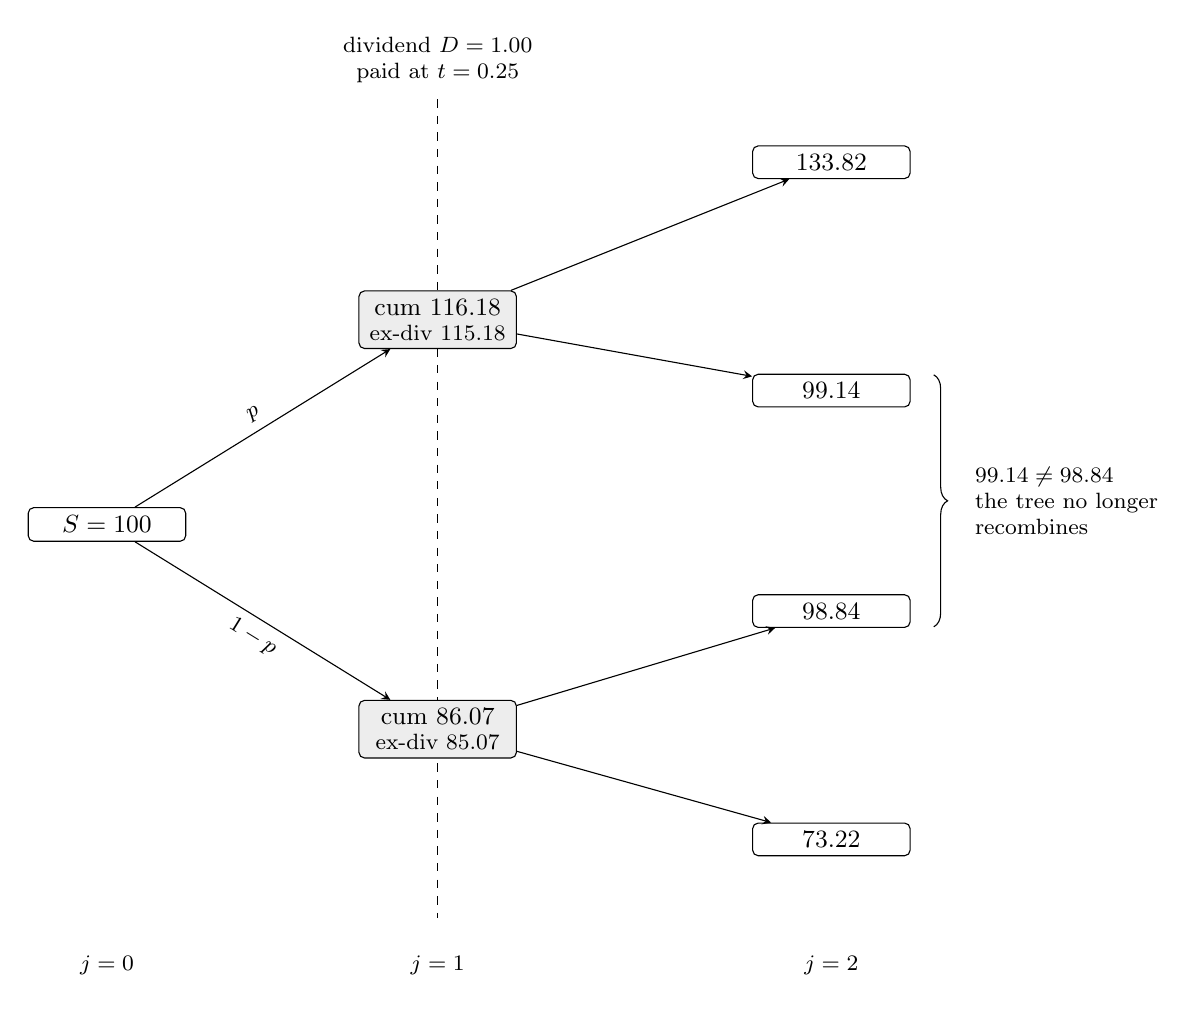
\begin{tikzpicture}[>=stealth,font=\small,
  nd/.style={draw,rounded corners=2pt,inner sep=3pt,minimum width=20mm,align=center},
  dv/.style={nd,fill=black!7}]
  \draw[dashed] (4.2,5.4) -- (4.2,-5.0);
  \node[nd] (s) at (0,0) {$S=100$};
  \node[dv] (su) at (4.2,2.6) {cum $116.18$\\[-2pt]\footnotesize ex-div $115.18$};
  \node[dv] (sd) at (4.2,-2.6){cum $86.07$\\[-2pt]\footnotesize ex-div $85.07$};
  \node[nd] (a) at (9.2,4.6) {$133.82$};
  \node[nd] (b) at (9.2,1.7) {$99.14$};
  \node[nd] (c) at (9.2,-1.1){$98.84$};
  \node[nd] (d) at (9.2,-4.0){$73.22$};
  \draw[->] (s) -- node[above,sloped,font=\footnotesize]{$p$}(su);
  \draw[->] (s) -- node[below,sloped,font=\footnotesize]{$1-p$}(sd);
  \draw[->] (su) -- (a); \draw[->] (su) -- (b);
  \draw[->] (sd) -- (c); \draw[->] (sd) -- (d);
  \node[font=\footnotesize,align=center] at (4.2,5.9) {dividend $D=1.00$\\paid at $t=0.25$};
  \draw[decorate,decoration={brace,amplitude=5pt}] (10.5,1.9) -- (10.5,-1.3);
  \node[align=left,font=\footnotesize,anchor=west] at (10.9,0.3)
    {$99.14 \neq 98.84$\\ the tree no longer\\ recombines};
  \node[font=\footnotesize] at (0,-5.6)   {$j=0$};
  \node[font=\footnotesize] at (4.2,-5.6) {$j=1$};
  \node[font=\footnotesize] at (9.2,-5.6) {$j=2$};
\end{tikzpicture}
\end{document}
